\section{Generating fractures from surfaces\label{sec:generating_fractures}}
To generate a realistic fracture we use the method of successive random additions described in \cref{chap:generating_surfaces,subsec:SRA_implementation} to generate random surfaces with a known Hurst exponent. We then displace the surfaces in the $z$-direction, so one is above the other, and let the space between the surfaces be the void\footnote{Since we are using periodic systems, we could also have let the space outside the surfaces be the fracture and get the same result. But for easier visualization and understanding we use the volume between the surfaces.}.

In practice we make a fractured silica structure using the following procedure
\begin{itemize}
    \item Prepare a slab of amorphous SiO$_2$.
    \item Generate two surfaces.
    \item Rescale the $(x,y)$-positions of surfaces so they span the molecular system.
    \item Rescale the $z$-values of the surfaces so all points are inside the system.
    \item Remove all atoms between the upper and lower surface.
\end{itemize}

The biggest problem with this procedure is removing the atoms between two surfaces. But since all points in both surfaces lie on a regular grid in the $x$-$y$-plane, there is a simple way of dividing the volume between the surfaces into tetrahedra. And checking if a point is inside a tetrahedra is a geometrical exercize that can be solved programmatically. If the two surfaces are not intersecting, we can divide the volume between them into convex hexahedra spanned out by the points
% \begin{align*}
%     (x^1_{i}, y^1_{i}), (x^1_{i+1}, y^1_{i}), (x^1_{i}, y^1_{i+1}), (x^1_{i+1}, y^1_{i+1}), \\
%     (x^2_{i}, y^2_{i}), (x^2_{i+1}, y^2_{i}), (x^2_{i}, y^2_{i+1}), (x^2_{i+1}, y^2_{i+1}),
% \end{align*}
\begin{align*}
    z(i,j)&, & &z(i+1,j),& & &z(i,j+1)&, &\text{and}& & &z(i+1,j+1)& & &\text{for} & &i,j \in [0,N)
\end{align*}
in the two surfaces (four points in each surface). We then divide each convex hexahedra into five tetraheda, as illustrated in \cref{fig:hex_to_tetra}, giving a total of $5(N-1)^2$ tetrahedra spanning the total volume between the two surfaces.
%
% We do this by utilizing the fact that the points in each heighmap lie on a regular grid in the $x$-$y$-plane. This means that we can divide the volume into tetrahedra, . If the two heightmaps are not intersecting, we see that we can divide the volume between them into convex hexahedra, one for each set of points
% ($x_{i}, y_{i}$), ($x_{i}, y_{i+1}$), ($x_{i+1}, y_{i}$), and ($x_{i+1}, y_{i+1}$) 
% % $(x_i, y_i)$  $(x_i, y_{i+1})$ $(x_{i+1}, y_i)$ $(x_{i+1}, y_{i+1})$
% in the $x$-$y$-grid. Each of these hexahedra can then be divided into five tetrahedra, as illustrated in \cref{fig:hex_to_tetra}.
%
% \begin{figure}[htpb]%
%     \centering%
%     
\includegraphics[width=0.4\textwidth]{images/fracture/hexahedron_to_tetrahedra.png}%
%     \caption{%
%         Illustration of how to divide a hexahedron into five tetraheda.%
%         \label{fig:hex_to_tetra}%
%     }%
% \end{figure}%
% %
% \begin{figure}[htpb]%
%     \centering%
%     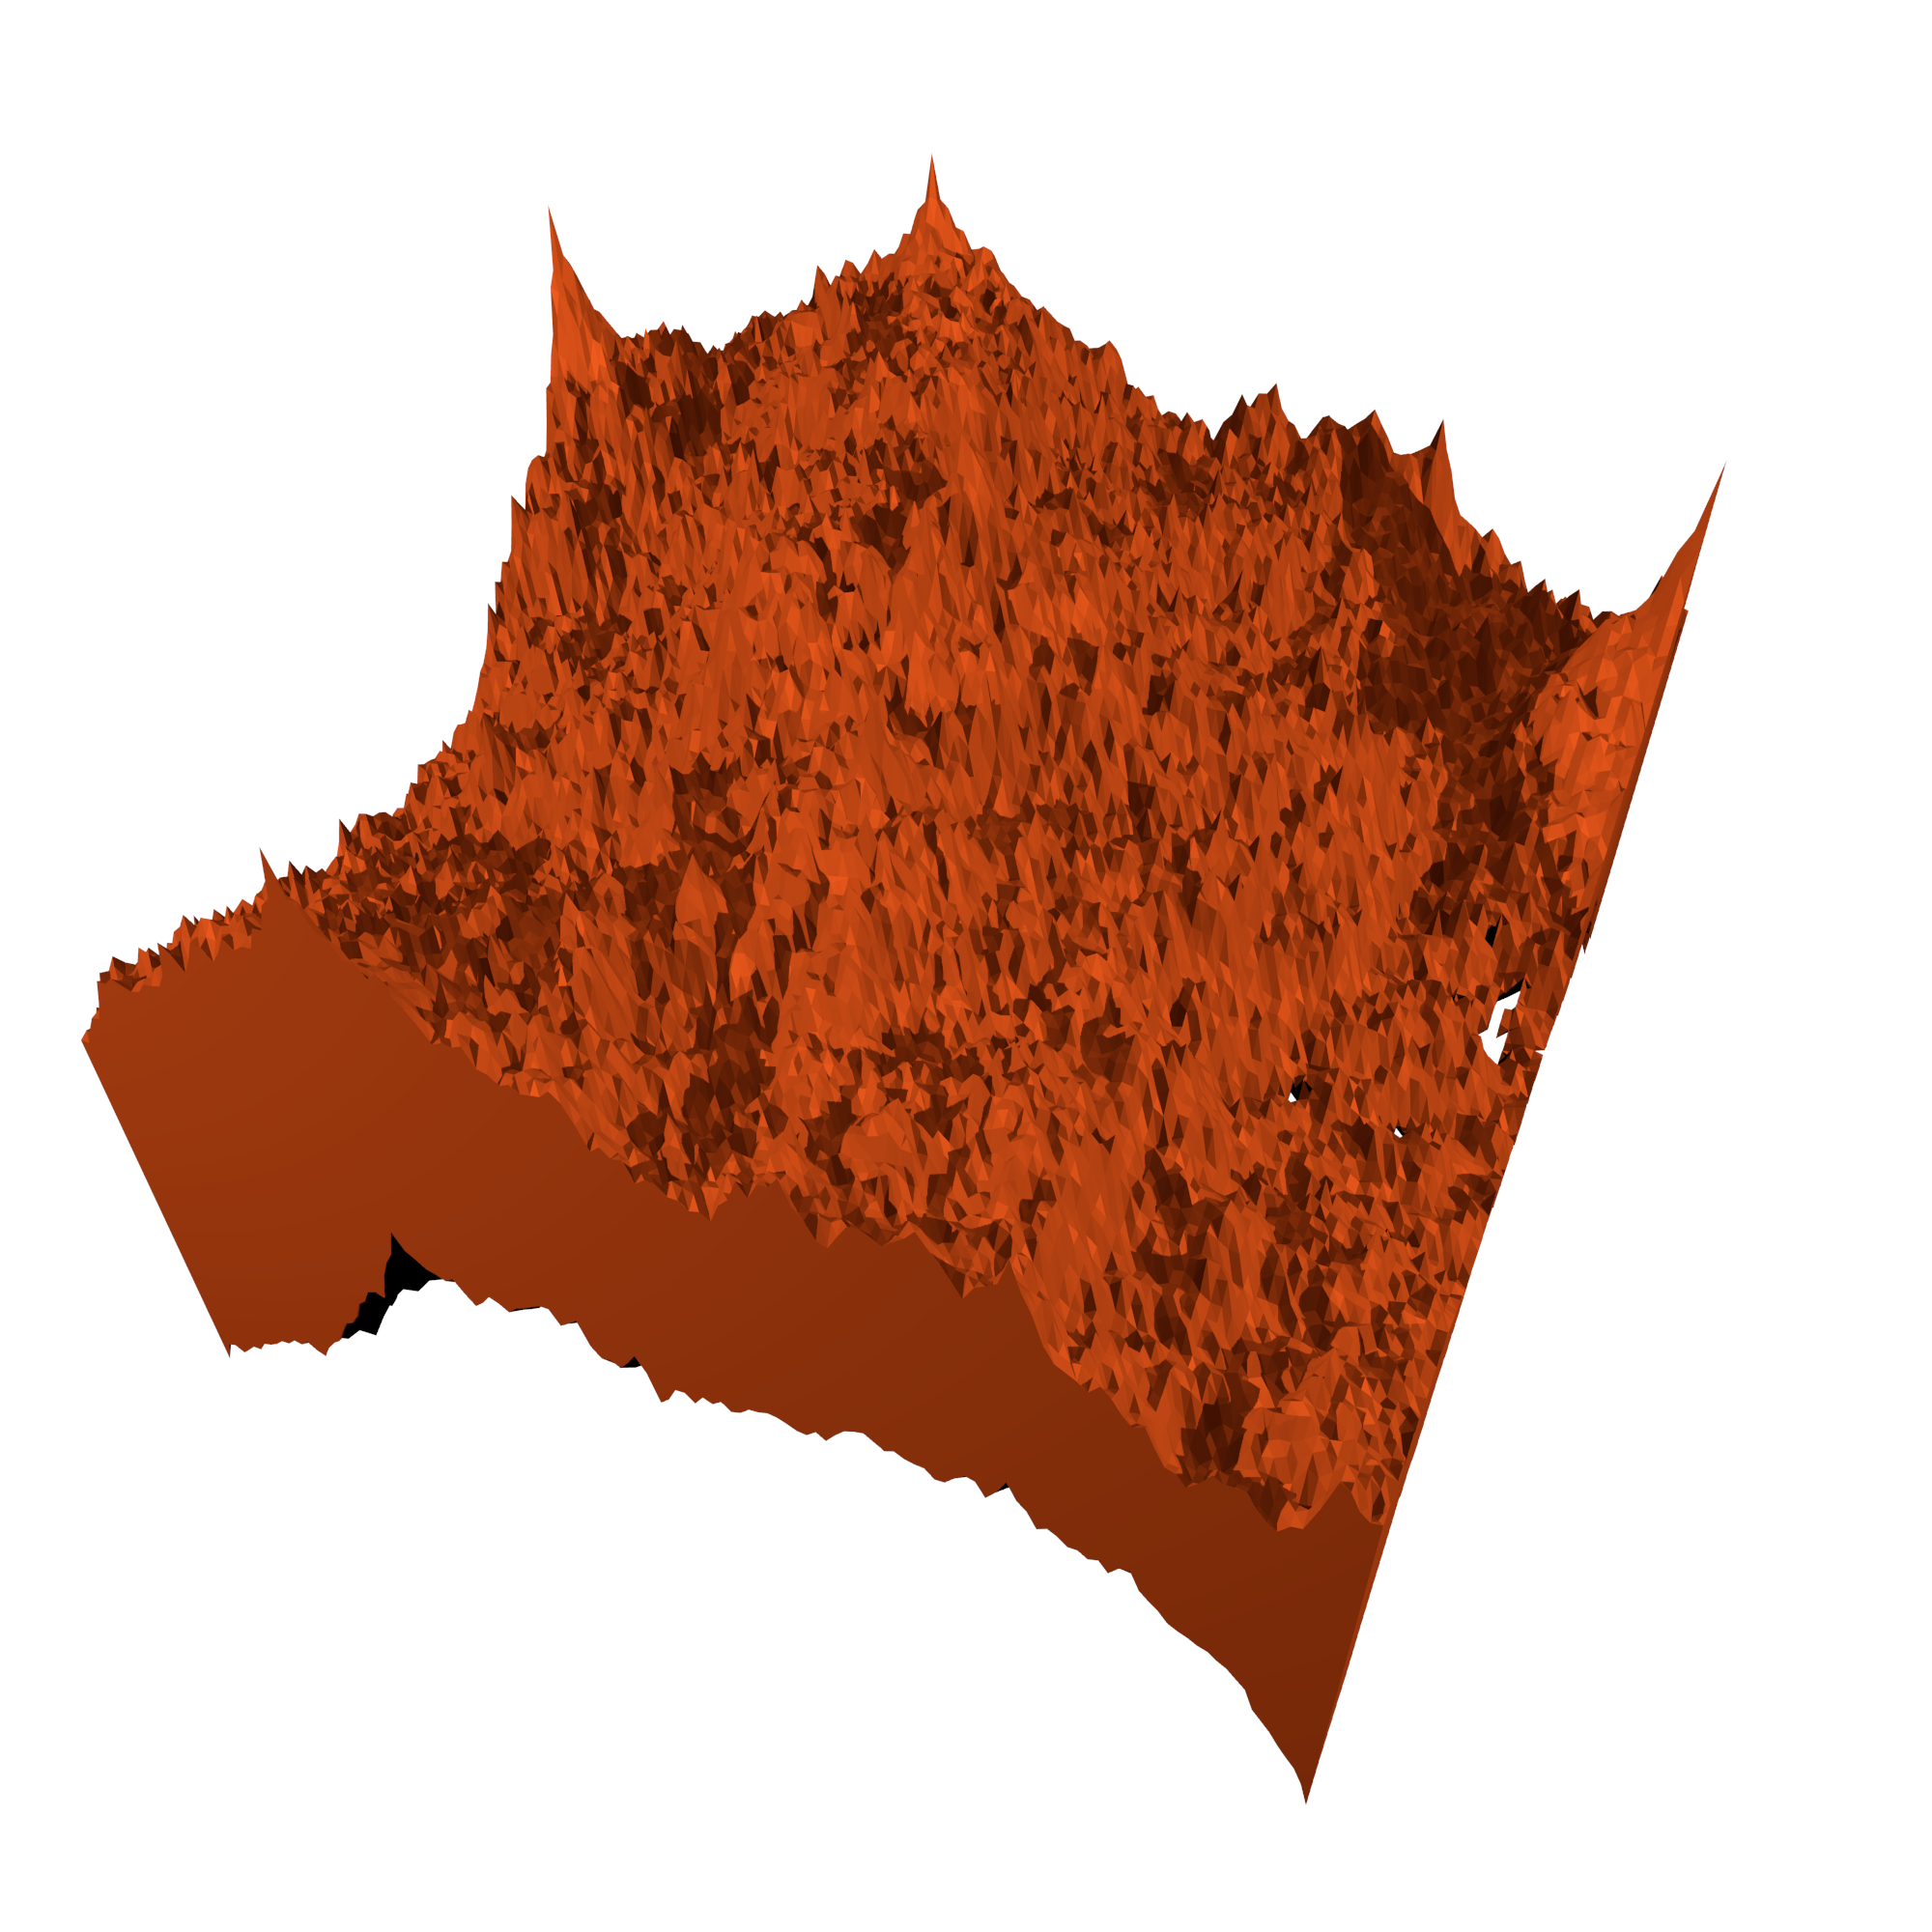
\includegraphics[width=0.6\textwidth]{images/fracture/fracture.png}%
%     \caption{%
%         A model of a fracture.%
%         \label{fig:fracture_model}%
%     }%
% \end{figure}%
%
\begin{figure}[htpb]%
    \centering%
    \setlength{\myfigwidth}{0.4\textwidth}%
%     \setlength{\mycaptionwidth}{0.3\textwidth}%
    \begin{subfigure}[b]{\myfigwidth}%
        \centering% % Need to center to get image centered over caption
        
\includegraphics[width=0.6\textwidth]{images/fracture/hexahedron_to_tetrahedra01_cycles_n200_cropped.png}%
        \caption{Illustration of how to divide a convex hexahedron into five tetraheda.}%
        \label{fig:hex_to_tetra}%
    \end{subfigure}%
    \hspace{0.1\textwidth}%
    \begin{subfigure}[b]{\myfigwidth}%
        \centering%
        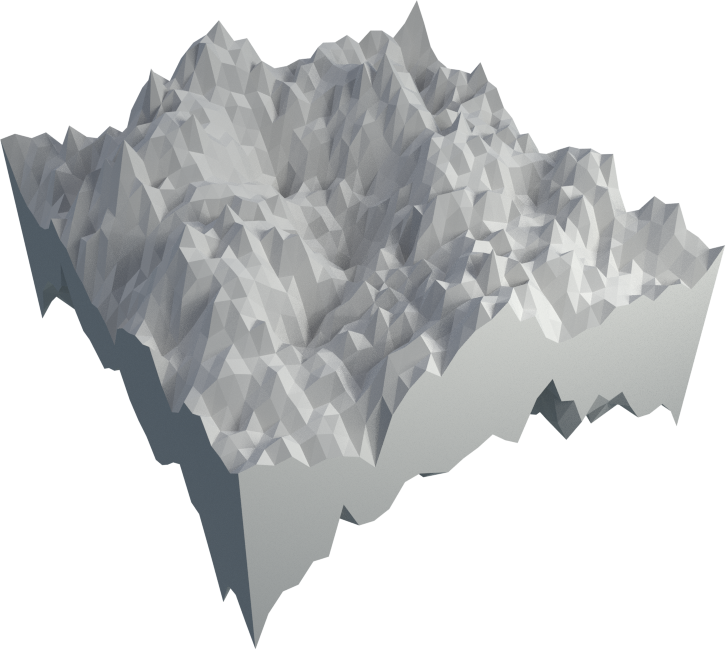
\includegraphics[width=\textwidth]{images/fracture/fracture05_n200_cropped.png}%
%         \includegraphics[width=\textwidth]{images/fracture/large_fracture04_300dpi_w20cm}%
        \caption{A random fracture made from two periodic surfaces.}%
        \label{fig:fracture_model}%
    \end{subfigure}%
\end{figure}%